\documentclass[border=10pt]{standalone}

\usepackage{tikz}
\usepackage{tikzsymbols}
\usetikzlibrary{calc,patterns,shapes.geometric}

\def\centerarc[#1](#2)(#3:#4:#5){\draw[#1] ($(#2)+({#5*cos(#3)},{#5*sin(#3)})$) arc (#3:#4:#5);}

\begin{document}
	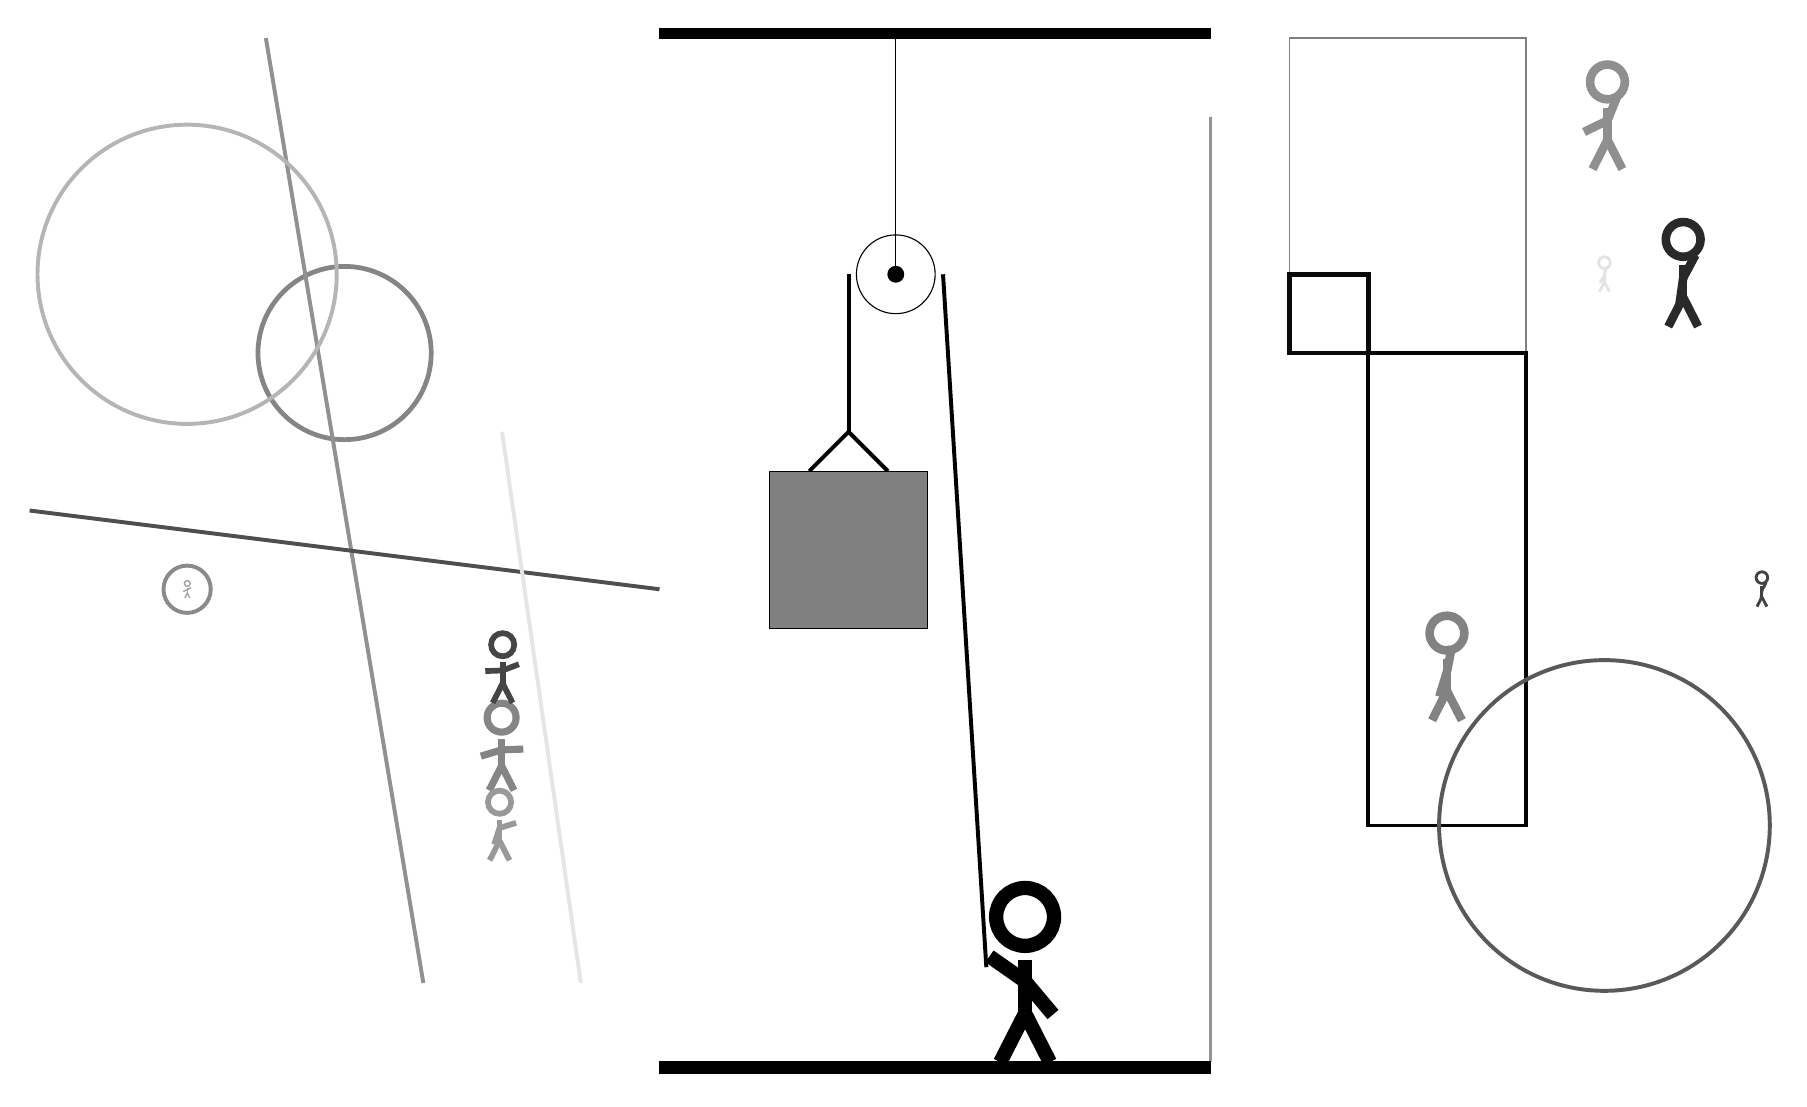
\begin{tikzpicture}
		%%%%% START %%%%%
		
		\draw[fill=black] (-2, 10) rectangle (5, 10.125);
		
		\draw (1, 7) circle (0.5);
		\draw[fill=black] (1, 7) circle (0.1);
		\draw (1, 10) -- (1, 7);
		
		\draw[line width=0.5mm] (-0.1, 4.5) -- (0.4, 5.0) -- (0.9, 4.5);
		\draw[fill=black!50] (-0.6, 4.5) rectangle (1.4, 2.5);
		
		\draw[line width=0.5mm] (0.4, 7) -- (0.4, 5.0);
		\centerarc[line width=0.5mm](1, 7)(0:180:0.6);
		\draw[line width=0.5mm](1.6, 7) -- (2.15, -1.8);
		
		\node at (2.6, -1.9) {\Strichmaxerl[10][-35][-50]};
		
		\draw [line width=0.5mm, color=black!46](-8, 3) circle (0.3);
		
		\draw [line width=0.6mm, color=black!48](-6, 6) circle (1.1);
		\node[line width=0.7mm, color=black!48] at (-4, 1) {\Strichmaxerl[5][17][2]};
		\node[line width=0.7mm, color=black!40] at (-4, 0) {\Strichmaxerl[4][72][17]};
		\draw[line width=0.4mm, color=black!42] (5, -3) rectangle (5, 9);
		\draw[line width=0.5mm, color=black!43](-7, 10) -- (-5, -2);
		\draw [line width=0.5mm, color=black!29](-8, 7) circle (1.9);
		
		\node[line width=0.2mm, color=black!84] at (11, 7) {\Strichmaxerl[6][82][62]};
		\draw[line width=0.2mm, color=black!50] (6, 10) rectangle (9, 6);
		\draw[line width=0.5mm, color=black!98] (7, 6) rectangle (9, 0);
		\draw [line width=0.5mm, color=black!65](10, 0) circle (2.1);
		
		\node[line width=0.7mm, color=black!49] at (8, 2) {\Strichmaxerl[6][73][79]};
		\node[line width=0.4mm, color=black!11] at (10, 7) {\Strichmaxerl[2][58][78]};
		
		\node[line width=0.7mm, color=black!44] at (10, 9) {\Strichmaxerl[6][26][68]};
		\node[line width=0.4mm, color=black!74] at (12, 3) {\Strichmaxerl[2][84][62]};
		\draw[line width=0.5mm, color=black!69](-2, 3) -- (-10, 4);
		\node[line width=0.3mm, color=black!73] at (-4, 2) {\Strichmaxerl[4][2][21]};
		\draw[line width=0.6mm, color=black!96] (7, 6) rectangle (6, 7);
		\draw[line width=0.5mm, color=black!10] (7, 4) rectangle (7, 4);
		\draw[line width=0.5mm, color=black!10](-4, 5) -- (-3, -2);
		\node[line width=0.3mm, color=black!36] at (-8, 3) {\Strichmaxerl[1][21][32]};
		
		
		\draw[fill=black] (-2, -3) rectangle (5, -3.15);
		
		%%%%% END %%%%%
	\end{tikzpicture}
\end{document}